\documentclass[a4paper,12pt]{extarticle}

\usepackage[T1]{fontenc}
\usepackage[utf8]{inputenc}
\usepackage{lmodern}

\usepackage[]{parskip}
\usepackage{hyperref, wrapfig, float, amsmath, adjustbox, array, pdflscape, soul, color, extsizes}
\usepackage{booktabs}
\usepackage{lscape}

\renewcommand{\arraystretch}{2}
\renewcommand{\contentsname}{Spis treści}
\renewcommand{\refname}{Bibliografia}
\renewcommand{\figurename}{Rys.}
\renewcommand{\tablename}{Tab.}

\usepackage{geometry}
\geometry{
  a4paper,
  margin=30mm,
  bottom=30mm
}

\usepackage{graphicx}
\usepackage[font=footnotesize,labelfont=bf,justification=centering]{caption}
\usepackage{subcaption}
\graphicspath{ {./images/}{../images/} }

\newcommand{\mathcolorbox}[1]{
  \begin{center}
    \colorbox{yellow}{$\displaystyle #1$}
  \end{center}
}
\newcommand{\pvec}[1]{
  \vec{#1}\mkern2mu\vphantom{#1}
}
\newcommand{\angstrom}{\mbox{\normalfont\AA}}

\begin{document}
  \onecolumn
  \begin{titlepage}
    \begin{center}
      \begin{figure}[H]
        \centering
        
\includegraphics[scale=.125]{logopp.png}
      \end{figure}
      \vspace*{.05\textheight}
      \huge\textbf{Politechnika Poznańska}\\
      \large\textbf{Wydział Inżynierii Materiałowej i Fizyki Technicznej}\\
      \large\textbf{Fizyka Techniczna}\\
      \vspace*{.2\textheight}
      \huge\textbf{Wytwarzanie i charakteryzacja warstw Langmuira i Langmuira-Blodgett}\\
      \vspace*{.025\textheight}
      \large\textbf{Jakub Bąbelek\\(nr.\ albumu: 136454)}
    \end{center}
  \end{titlepage}

  \tableofcontents
  
  \clearpage

  \section{Wstęp}
  \subsection{Surfaktanty}
  Surfaktanty to substancje powierzchniowo czynne
  (z ang. \textbf{surf}ace \textbf{act}ive \textbf{a}ge\textbf{nt}), gromadząc
  się na granicy faz, znacząco zmienia właściwości powierzchniowe cieczy,
  w której jest rozpuszczona. Należą do szerokiej klasy substancji zwanych
  amfifilami które ze względu na swoją asymetryczną budowę wykazują odmienne
  zachowanie w stosunku do faz polarnych i niepolarnych.

  \subsection{Warstwy Langmuira}
  Monowarstwy molekularne tworzone na granicy faz ciekłej i gazowej nazywamy
  warstwami Langmuira. Tworzą je powierzchniowo aktywne związki organiczne,
  wytwarza się je poprzez nakroplenie odpowiedniej ilości substancji badanej
  na ciecz (najczęściej woda destylowana --- w laboratorium używany jest system
  MilliQ). Po odparowaniu rozpuszczalnika na powierzchni cieczy pozostaje monowarstwa
  molekularna substancji badanej którą dzięki konstrukcji wanny
  (\figurename\ref{fig:wanna}) ściskamy za pomocą dwóch hydrofobowych barier co
  umożliwia nam pomiar ciśnienia powierzchniowego w funkcji powierzchni dostępnej
  dla jednej molekuły (do tego pomiaru wykorzystuje się płytkę Wilhelma).

  \begin{figure}[H]
    \centering
    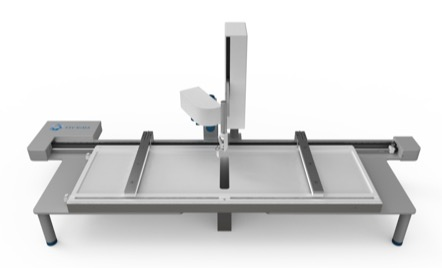
\includegraphics[width=12cm]{wanna.jpg}
    \caption{Wanna Langmuira}
    \label{fig:wanna}
  \end{figure}

  \subsection{SAM}
  Samoorganizujące monowarstwy organicznych molekuł tworzące się spontanicznie
  na powierzchni dzięki adsorbcji, tworzą uporządkowane domeny.

  \section{Dane i obliczenia}
  \begin{table}[H]
    \centering
    \begin{tabular}{c|cc}
    \toprule
    \textbf{Substancja nanoszona}            & R1646                          & Kwas stearynowy                \\
    \midrule
    \textbf{Masa cząsteczki}                 & \( 717 \frac{g}{mol} \)        & \( 284.5 \frac{g}{mol} \)      \\
    \textbf{Objętość wkroplona}              & \( 30 \mu l \)                 & \( 90 \mu l \)                 \\
    \textbf{Stężenie}                        & \( 10^{-3} \frac{mol}{dm^3} \) & \( 10^{-3} \frac{mol}{dm^3} \) \\
    \textbf{Powierzchnia pomiędzy barierami} & \multicolumn{2}{c}{\( 23250 mm^2 \)}                            \\
    \bottomrule
    \end{tabular}
  \end{table}

  Ilość molekuł naniesionych na powierzchnię wody obliczamy ze wzoru (\ref{eq:ilosc})
  \begin{equation}
    N = \frac{V C}{M} N_A = \frac{V C_{mol} M}{M} N_A = V C_{mol} N_A
    \label{eq:ilosc}
  \end{equation}
  \begin{center}
    \tiny{gdzie:
    \( V\ -\ objętość\ wkroplona,\ 
    M\ -\ masa cząsteczki,\ 
    C\ -\ stężenie\ badanej\ substancji\ w\ rozpuszczalniku,\ 
    C_{mol}\ -\ stężenie molowe,\ 
    N_{A}\ -\ liczba Avogadra \)}
  \end{center}

  \begin{table}[H]
    \centering
    \begin{tabular}{c|cc}
    \toprule
    \textbf{Substancja} & R1646                   & Kwas stearynowy           \\
    \midrule
    \textbf{N}        & \( 1,807 * 10^{16} \) & \( 5,419 * 10^{16} \) \\
    \bottomrule
    \end{tabular}
  \end{table}

  Powierzchnię dostępną dla pojedynczej molekuły po nakropleniu obliczamy ze wzoru (\ref{eq:pow})
  \begin{equation}
    A = \frac{S}{N}
    \label{eq:pow}
  \end{equation}
  \begin{center}
    \tiny{gdzie:
    \( S\ -\ Powierzchnia\ pomiędzy\ barierami,\ 
    N\ -\ ilość\ molekuł\ (\ref{eq:ilosc}). \)}
  \end{center}

  \begin{table}[H]
    \centering
    \begin{tabular}{c|cc}
    \toprule
    \textbf{Substancja}     & R1646                   & Kwas stearynowy           \\
    \midrule
    \textbf{A}             & \( 1,29 * 10^{-17} [m^2] \) & \( 4,29 * 10^{-18} [m^2] \) \\
    \bottomrule
    \end{tabular}
  \end{table}

  \clearpage
  %
  %Ściśliwość obliczamy ze wzoru (\ref{eq:scis}) dla wartości przegięcia
  %\begin{equation}
  %  \beta = -\frac{1}{A} \left( \frac{dA}{d\pi} \right)
  %  \label{eq:scis}
  %\end{equation}
  %\begin{center}
  %  \tiny{gdzie:
  %  \( \pi\ -\ napięcie\ powierzchniowe,\ 
  %  A\ -\ powierzchnia\ dost.\ dla\ jednej\ molekuły\ (\ref{eq:pow}). \)}
  %\end{center}
  %
  %\begin{table}[H]
  %  \centering
  %  \begin{tabular}{c|cc}
  %  \toprule
  %  \textbf{Substancja} & R1646                   & Kwas stearynowy           \\
  %  \midrule
  %  \textbf{\( \beta \)} & \( 1,29 * 10^{-17} [m^2] \) & \( 0.08351 [\frac{m}{mN}] \) \\
  %  \bottomrule
  %  \end{tabular}
  %\end{table}

  \begin{figure}[H]
    \centering
    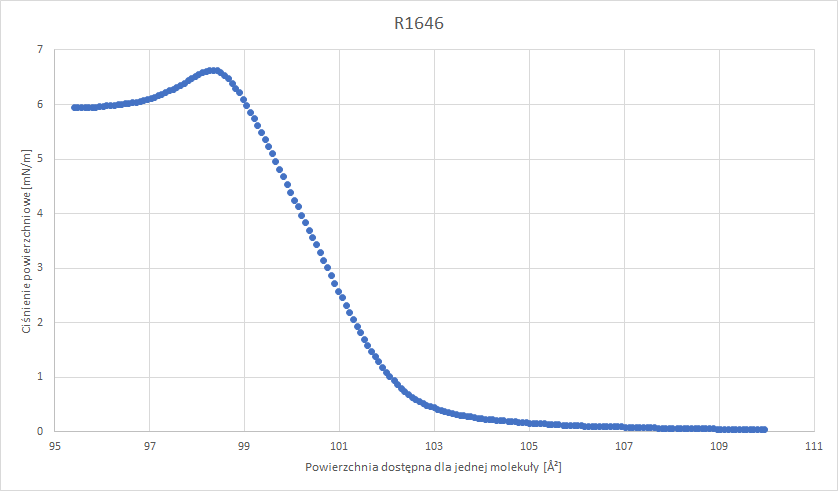
\includegraphics[width=10cm]{r1646.png}
    \caption{Ciśnienie powierzchniowe od powierzchni dostępnej dla jednej cząsteczki --- R1646}
    \label{fig:r1646}
  \end{figure}

  \begin{figure}[H]
    \centering
    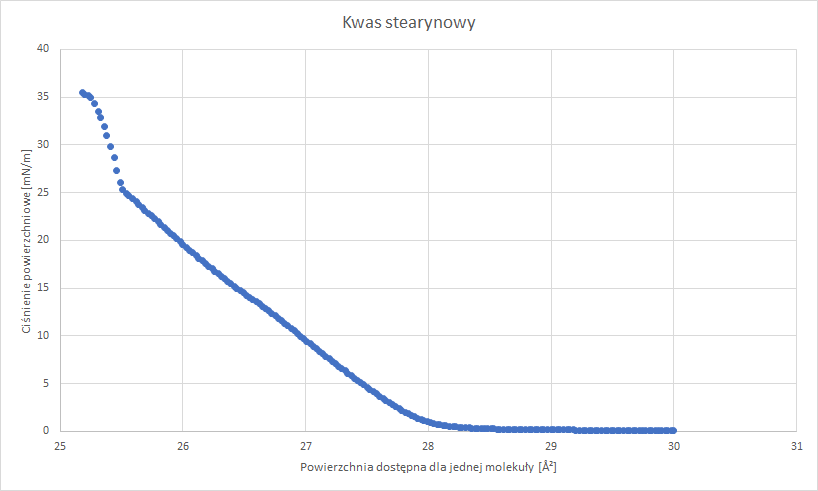
\includegraphics[width=10cm]{kwas.png}
    \caption{Ciśnienie powierzchniowe od powierzchni dostępnej dla jednej cząsteczki --- Kwas stearynowy}
    \label{fig:kwas}
  \end{figure}

  Następnie z wykresów odczytujemy wartości \( A_C,\ A_{EXT},\ A_{0},\ \pi_C \)

  \begin{table}[H]
    \centering
    \begin{tabular}{c|cc}
    \toprule
    \textbf{Substancja} & R1646 & Kwas stearynowy \\
    \midrule
    \textbf{\( A_C \)}     & \( 98,43 \)  & \( 25,2 \)  \\
    \textbf{\( A_{EXT} \)} & \( 102,69 \) & \( 28,09 \) \\
    \textbf{\( A_{0} \)}   & \( 109,19 \) & \( 29,28 \) \\
    \textbf{\( \pi_C \)}   & \( 6,15 \)   & \( 35,3 \)  \\
    \bottomrule
    \end{tabular}
  \end{table}

  \section{Wnioski}
  Wartości otrzymane doświadczalnie są zbliżone do wartości teoretycznych,
  nie są jednak idealne co mogło zostać spowodowane przez czynniki zewnętrzne tj.
  ciśnienie atmosferyczne, temperatura oraz szybie tempo przeprowadzanego doświadczenia
  ze względu na ograniczenia czasowe. Metoda przeprowadzania doświadczenia
  pozwala na szybkie i łatwe uzyskanie monowarstw molekularnych jednak do uzyskania
  dokładnych wyników potrzebna jest izolacja układu od czynników zewnętrznych.

\end{document}